\documentclass[12pt,letterpaper]{article}
\usepackage{fullpage}
\usepackage[top=2cm, bottom=4.5cm, left=2.5cm, right=2.5cm]{geometry}
\usepackage{amsmath,amsthm,amsfonts,amssymb,amscd}
\usepackage{lastpage}
\usepackage{enumerate}
\usepackage{fancyhdr}
\usepackage{mathrsfs}
\usepackage{xcolor}
\usepackage{graphicx}
\usepackage{listings}
\usepackage{hyperref}

\hypersetup{%
  colorlinks=true,
  linkcolor=blue,
  linkbordercolor={0 0 1}
}
 
\renewcommand\lstlistingname{Algorithm}
\renewcommand\lstlistlistingname{Algorithms}
\def\lstlistingautorefname{Alg.}

\lstdefinestyle{Python}{
    language        = Python,
    frame           = lines, 
    basicstyle      = \footnotesize,
    keywordstyle    = \color{blue},
    stringstyle     = \color{green},
    commentstyle    = \color{red}\ttfamily
}

\setlength{\parindent}{0.0in}
\setlength{\parskip}{0.05in}

% Edit these as appropriate
\newcommand\course{Statistics I}
\newcommand\hwnumber{2.4}                  % <-- homework number
\newcommand\NetIDa{Atreya Choudhury}           % <-- NetID of person #1
\newcommand\NetIDb{bmat2005}           % <-- NetID of person #2 (Comment this line out for problem sets)

\pagestyle{fancyplain}
\headheight 35pt
\lhead{\NetIDa}
\lhead{\NetIDa\\\NetIDb}                 % <-- Comment this line out for problem sets (make sure you are person #1)
\chead{\textbf{\Large Assignment \hwnumber}}
\rhead{\course \\ \today}
\lfoot{}
\cfoot{}
\rfoot{\small\thepage}
\headsep 2em

\begin{document}
\textbf{Question:}
\textit{Consider the following sample data set.}
\begin{center}
  121 171 158 173 184 163 157 85 145 165 172 196 170 159 172 161 187 100 142 166 171
\end{center}

\begin{enumerate}[1.] \setlength{\itemsep}{30pt}
  \item \textit{What is the median?}
  
  \textbf{\textit{Answer: }}
  
  The median is \textbf{163}
  \item \textit{What are the upper and lower quartiles?}
  
  \textbf{\textit{Answer: }}

  Lower quartile: \textbf{157}

  Upper quartile: \textbf{172}
  \item \textit{Construct a box plot for the data.}
  
  \textbf{\textit{Answer: }}

  \begin{figure*}[h]
    \centering
    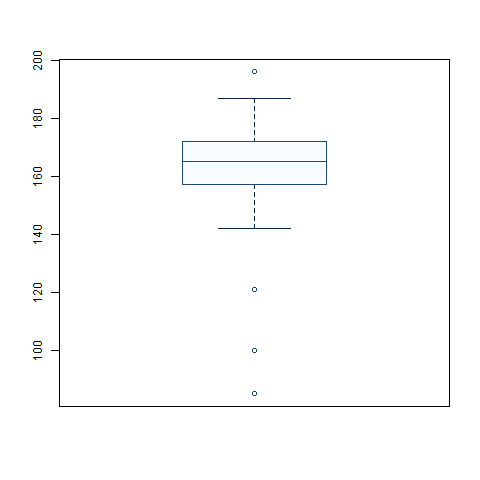
\includegraphics[width=9cm]{box-plot.png}
    \caption{Box Plot of Given Data}
  \end{figure*}
  \newpage
  \item \textit{Identify the values, if any, that are outside the 1.5 IQR limits from the quartiles.}
  
  \textbf{\textit{Answer: }}

  The values, \textbf{85}, \textbf{100}, \textbf{121} and \textbf{196} lie outside the 1.5 IQR limits from the quartiles.
  \item \textit{Is the distribution of the data symmetric, skewed to the left or skewed to the right?}
  
  \textbf{\textit{Answer: }}

  The mean of the data is 158 and the median is 165.
  As the median is greater than the mean, we can conclude that the data is \textbf{skewed to the left}.
\end{enumerate}
\end{document}